\chapter{Discussion}
\label{chpt:discussion}
This chapter will review the choices that have been made throughout the project, while reflecting on other possible choices and what consequences they would have on the product.

\section{Requirements}\label{sec_disc_requirements}
A set of requirements was specified and categorised as either must have, good to have or stretch goals. Two requirements were categorised as must have: \textit{Object Recognition} and \textit{Target Tracking}.

The requirement of \textit{Object Recognition} is fulfilled trough \gls{opencv} which makes it possible to recognise a predefined object, by the use of template matching. 

The rig was built in order to provide the Lego Mindstorms motors with a base of which they can perform horizontal and vertical rotations, to move a laser around to point in specified directions in the room, in which it is located.
The \gls{nxt} controls these motors and can thereby adjust the direction of the laser, and therefore track the recognised object by aiming the laser at the object.
By doing combining these elements the second requirement, \textit{Target Tracking}, has likewise been fulfilled.

Advanced Target Acquisition have not been implemented in the system. However, the system accepts position information in a general form, meaning the changes that are to be done for the system to accept positions from more than two cameras is minimal. By including this option new obstacles are introduced, as the system would have to discard redundant information, as there are more candidates to specify the object's position. Information can be deemed redundant if the position it specifies is too distant from the set of collected positions. This situation can occur if a camera recognises a wrong object or somehow corrupt the data it sends. Furthermore, by having more candidates, the information can be evaluated, to find possible errors.

\section{Hardware}\label{sec:disc_hardware}
The choice of hardware have brought different implications and restrictions on what is possible when designing the system. Some of these implications could have been avoided by using different pieces of hardware, but these devices would have their own restrictions as well. This section will discuss the possibilities and restrictions of altering the hardware choices and setup.

\subsection{Mindstorms Devices}\label{subsec:disc_minds}
The \gls{nxt} is used to calculate the angles that the rig adjust itself to when instructed to point at a target, and the \gls{rsp} is responsible for the analysis of images from the camera video streams. There is a newer version of the nxt called \gls{ev3}. If the newer Mindstorms brick was used, it would be possible to offload the calculations from the \gls{rsp} to the brick as it has more computational power. As seen in \cref{tbl:ev3_spec} the \gls{ev3} has a faster processor along with a large increase in the amount of memory it has access to. It should be noted that the power consumption is increased as well.

\begin{table}[ht]
  \centering
  \begin{tabular}{|l|r|}
  \hline
    Main processor & 32-bit ARM9 processor, Texas Instrument AM1808\\ \hline
    Memory & 64 MB DDR RAM, 16 MB FLASH, 256 KB EEPROM\\
  \hline
  \end{tabular}
  \caption{Summarised \gls{ev3} intelligent brick specification\cite{ev3_specs}}
  \label{tbl:ev3_spec}
\end{table}

By offloading these calculations to the \gls{ev3} it would be possible to replace the \glspl{rsp} with a simpler device, which transfers the video stream directly to the \gls{ev3}. This solution will also allow the system to spare the laptop as it will not be necessary to have an intermediate component to act as modem.

\subsection{No PC and Lego Mindstorms NXT Solution}\label{subsec:disc_no_pc_lego}
In the current system setup, a total of three different devices are used, namely a \gls{nxt}, \gls{rsp} and a laptop, each running a different \gls{os}. If a newer version of the \gls{rsp} was used, such as the \gls{rspz}, it would be possible to create a system of unified devices which would widen the communication possibilities. The \gls{rspz} is a cheap embedded device with normal and mini USB ports and can be modified to connect trough an Ethernet connection as well. The \glspl{rsp} have their own set of motors which is found in a varying price and quality range, which could be used instead of the Lego Mindstorms motors.\cite{rs_pi_zero} \cite{rsp_zero_ethernet}

If the system, besides the sensors and actuators, only consisted of \glspl{rspz}, the communication process would be simplified, since the amount of different \glspl{os} and devices the project group would have to familiarise themselves with would be reduced.

\subsection{Modern Camera Possibilities}\label{subsec:disc_modern_cam}
%Newer cameras will allow better precision and the object reg will be more effective
%	(Bedre template - små objekter - chance for rigtigt - ansigtsgenkendelse)
In \cref{ss:cam_type} two camera options are presented and as stated the \acrfull{cvbw3} is selected. However, since the release of \gls{cvbw3}, the quality of webcams have been enhanced, including the quality of the images. This quality increase manifests itself in higher resolution, a larger point of view and a higher degree of details in images.

These quality enhancements are relevant in relation to object recognition as presented in \cref{ch:obj_rec}. This is due to the higher degree of details in an image as it makes it easier to distinguish elements, resulting in easier object detection and recognition.

\subsection{Multiple Cameras per Raspberry Pi}\label{subsec:disc_mult_pi}
%Why not use two or more cams per PI? (answer: ram)
As the system is designed, each camera unit is constructed using a \gls{cvbw3} and a \gls{rsp}, both presented in \cref{chp:tech}. An alternative setup would be to equip each \gls{rsp} with multiple \glspl{cvbw3}. There are both advantages and disadvantages to such a solution. The advantage is a decrease in the amount of hardware needed in total, as two cameras can be connected to a single \gls{rsp}, such that it is possible to half the amount of \glspl{rsp} needed. However there is a disadvantages to this approach in relation to the range of the cameras units. This is due to the USB specification, which states that a USB cable's length should at maximum be 5 meters, otherwise a decrease in transfer speed may occur \cite{usb_spec}. While a Ethernet cable can be up to 100 meters before a decrease in transfer speed may occur. By using two cameras per \gls{rsp}, the amount of hardware per unit will decrease, but more units are needed to cover the same area.

\subsection{Alternative Motor}\label{subsec:disc_step}
The motors used are \glspl{dcm} which are controlled by regulating the voltage they receive. As a consequence of this method it is not possible, by standard, to instruct the motor to rotate a set amount of degrees. Therefore a \gls{pid} has been implemented in order to rotate the correct amount of degrees. It would be possible to avoid the implementation of a \gls{pid} if a step motor was used, as it can be instructed to rotate a set amount of steps. It would simplify the implementation and make the system react faster as it would not have to call a \gls{pid} function when instructed to rotate. However, step motors are generally very expensive when compared to their \glspl{dcm} counterpart. 

\section{Implementation}\label{sec:disc_implementation}
When implementing the mathematical formulas and getting them to work with a real life environment, different problems arise which have to be handled. One of these comes from how the rig has been designed and what that entails. How the object recognition have been implemented also provides a set of dilemmas when working with multiple cameras.

\subsection{Rig Design}\label{subsec:disc_rig}
When calculating the angles, there is an offset that has to be considered because of how the rig is constructed. There are two axes each represented by a motor which is used to angle the laser in the right direction when an object has been targeted. \Cref{fig:rig_flat} from \cref{sc:rig} shows where the offset is. From the turret base vertical centre line, the centre of the big gear, to the axis that makes the vertical rotation there is a distance of 6,4cm which form the offset.

If the rig was build in such a way such that the two axes had the same rotational point, it would not be necessary to include an offset in the calculations. This can be achieved by using a gimbal setup with the laser in the centre.

\begin{figure}[H]
  \centering
  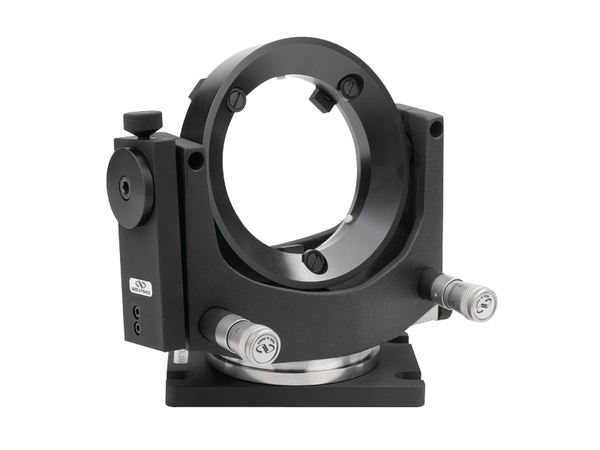
\includegraphics[width=0.80\textwidth]{graphics/discussion/gimbal.jpg}
  \caption{Gimbal example\cite{gimbal}}
  \label{fig:gimbal}
\end{figure}

If the laser was fastened in centre of the gimbal from \cref{fig:gimbal}, it would be possible to eliminate any offsets if the coordinate system would have its base in the centre as well. This would simplify the angle calculations and make them more precise, as the possible imprecisions made when measuring the offset will be eliminated as well.

\subsection{Multiple Camera Tracking Dilemma}\label{subsec:disc_mult_cam}
In order to find and track an object with the current setup, it is necessary that all connected cameras have targeted the same object. If one or more cameras are unable to target the same objects as the other cameras, the result is undefined. What will probably happen is that the calculated angle on the \gls{nxt} will be inequivalent with the angle of the correct target. If a camera unit is unable to find and target an object, the pixel offset is undefined, which will cascade to the following calculations. When an objects position is calculated on the \gls{nxt}, all the information retrieved from the pc is used, which means if one of them delivers erroneous or otherwise nonsensical data the calculations will be inaccurate.

This could be avoided if the \gls{nxt} was able to discard results that are over a set margin in order to weed out said erroneous data. By discarding wrong data the \gls{pid} will be faster and more precise as it will no longer have to rotate towards a wrong direction, and instead it can use the most recently accepted data packet.

%Simon har læst hertiltiltiltiltiltil. ok siiiimon xD
\section{Test}
\label{sec:disc_test}
\Cref{chpt:motor_test} covers the tests that was conducted with the activators that are used with the rig, but contains no references to the sensors which have been used in the project. The cameras are the choice of sensors when an object has to be recognised and tracked, it would therefore be beneficial for the project to test the quality and limit of these cameras. The produced software have not been tested either, besides small simplistic undocumented test made to ensure that bits and parts gave expected results while they were still being developed. The following sections will describe which additional tests that could have been beneficial for the project.

\subsection{Camera}\label{subsec:disc_camera}
The tests made on the cameras will help to estimate the quality and thereby the chance of the finding the right objects when executing the object recognition software.

Four tests were considered for the cameras where each test would cover different aspects of the devices usability. The four tests were:
\begin{itemize}
\item Verification test of the \gls{fov}
\item Test of the how well cameras fares in different light levels
\item Test of picture noise
\item Test of picture frame rate consistency
\end{itemize}

The Verification test of the \gls{fov} is relevant as the target tracking calculations is dependent on this property. If these calculations returns incorrect angles, it can prove difficult to find where the mistakes were made since no tests have been conducted, and it is therefore not possible to exclude the possibility of having a wrong \gls{fov} constant. The test setup would be to place a camera a set distance, 2-3 meters, away from a blackboard. The camera should point at the centre of the board, and the board should face the camera such that a 90\degree angle from the board would point at the centre of the camera lens. The board will then be chalked up with vertical lines representing where the camera should be able to see within its \gls{fov}. The camera then takes a picture which will be inspected, and if the lines is not in the outskirts of the picture additional lines should be made with a set amount of degrees between them so the actual \gls{fov} can be measured.

The test that inspects how well the cameras fares in different light levels would be helpful as the light level will affect how the colour recognition performs. If it is much darker or lighter than what it is in the template it can be unable to find the target. The template is the reference picture of the object it has to find. It is possible to create many test scenarios that concerns itself with different kind of light setup which test many different aspects of the object recognition. The test that was considered would focus on colour aspect as the light source would be the same, but the light level would be different from what it was at the time the template picture were made. The test setup would be to place the object at the same location that the template picture were taken at, and the keep adjusting the lighting level so keeps getting darker. A camera would point at the object and a device will execute the object recognition software on the video stream. When it no longer is able to consistently find the object, the light level will be noted.

The test of picture noise would be beneficial, as it would provide insight in what techniques that should be used to counter the level of noise present in the pictures. The techniques will complicate the object recognition as more steps are required in order to recognize the correct object. The setup would involve placing the camera in a room where the environment is static in the sense that nothing is moved in between the frames. It is important that the camera is standing still and that the light level stays the same as these factors will affect the result of the comparison made between the frames. The comparison is between two or more frames where each pixel in said frames is compared in order to spot differences. The pixel differences is then counted and compared to the total pixel count in a frame to calculate the \textperthousand difference.

The last test with the cameras would be to test the frame rate consistency. In other words, to check if the time frame between each transfer to the connected device is the same. The consistency is important when calculating a \gls{rta} as any inconsistencies will affect the rate which the devices connected to the cameras can perform their calculations and transfer that data. The test setup would be to connect a camera to a device. The device would then execute a program that timestamps the frames it receives from the video stream. The timestamps would then be compared to find any inconsistencies between the time it takes to receive each picture from the stream.

\subsection{Motor Test}\label{subsec:disc_motor}
in \cref{chpt:motor_test} one test was described and the results was analysed. One problem with this test was that two possible error sources could have affected the standard deviation, as presented in \cref{subsec:con_speed}. Therefore it could be beneficial to conduct two more tests; one for testing the internal tick counter and one for testing the size and speed under constant voltage.

It would be prudent to perform the Speed-Timing Test, where the test setup is connect to a power source where a constant voltage is guaranteed, and not a power source which discharges over time. Such a test could determine the effect a constant power source have on the test results. If it turns out that a constant voltage removes the linear growth in standard deviation, other tests could be a benefit to conduct. The effect of lowering the voltage could systematically be tested so it was known how the motor performs at given voltage.

Another aspect is to test if the battery pack used in the test could oscillate so much it would be observable in the standard deviation. This should be done such that it is understood how the battery pack charges and discharges, and by such the battery based power source influence on the recorded test results. These results should be combined with the results of testing with constant voltage in order to conclude the effect of the standard deviation.

The last test to conduct is to compare the internal tick counter with how far the motors actually turns. The motors have an intern tick counter which counts how many degrees it have turned around its axis. The counter should be that one tick correspondence one degree. The counter is used when turning the laser and will therefore affect how well it will be able to point at a target. The test setup would be to have extra equipment to measure the degrees turned and compare it with the tick counter. If there is a constant risk of skipping it can be observed in the results.


\subsection{Software Test}\label{subsec:disc_software}
During the system development phase, no structured software test were implemented. However it would be an advantage to implement structured test of the source code, as this would make it possible to prove the correctness of the source code. Using test coverage tools developers and testers could get an overview over the parts of the source code which are not yet tested, and which parts of the source code that already are included in the structured tests.

If a structured software test is implemented, it would not only make it possible to prove the correctness and provide test coverage of source code. A structured test would also enable quality control of the source code, thus ensuring the source code lives up to certain quality control attributes. Implementing a comprehensive quality control procedure is an greatly excessive undertaking, but should result in a better product as it would uphold certain criteria and quality control attributes.